\chapter{Introduction}
\label{sec:introduction}

Many scientific experiments are run in sequence. An experimenter performs one
measurement, updates their belief about the system, and uses that belief to choose the
next measurement. When each measurement is expensive and prior knowledge is broad, the
order and content of these choices determine how quickly the experimenter learns.
Sequential Bayesian experimental design (BED) is the formal framework for making them.
At each step it selects the experiment expected to be most informative about the
unknown parameters of the system, where informativeness is measured by the expected
information gain, the expected reduction in posterior uncertainty about the
parameters~\citep{lindley1956measure,chaloner1995bayesian,ryan2016review,rainforth2024modern}.

This setting is becoming central across the natural sciences and engineering, and in
particular for systems described by dynamics that unfold over time. In wastewater
treatment, cell-free biosynthesis, dynamic metabolism, bioprocess control, and battery
cycling, the same total input can produce very different outcomes depending on when it
is applied~\citep{henze2000activated,silverman2020cellfree,martin2023dynamic,espinelrios2024cybergenetics,vanvlijmen2025battery}.
Recent experimental work makes the point concrete. Timed inputs to an enzymatic
reaction cascade can raise yields well above conventional all-at-once
dosing~\citep{jakstaite2026timedbatch}, and actively designed perturbations can control
intricate reaction networks that fixed protocols cannot~\citep{vansluijs2024iterative}.
Choosing not only how much to intervene but when turns experimental design into a
sequential control problem over a large, history-dependent space of input schedules,
which is precisely the regime sequential BED is meant to handle.

The systems where this matters most are also the hardest for design algorithms, and
the difficulty has a specific shape. They are modelled by stiff ordinary differential
equations (ODEs), so the numerical solution is sensitive and the solver is expensive.
Their kinetic parameters are known only to within several orders of magnitude, so the
prior is broad. And because the dynamics are highly responsive to those parameters, a
single well-placed measurement can carry many nats of information. Each of these
properties is individually manageable, but their combination is exactly where current
amortized design methods break down. This thesis identifies why they break down, and
proposes a method that does not.

\section{The saturation obstacle}
\label{sec:intro-obstacle}

Two families of methods dominate modern sequential BED, and both struggle on this
regime for different reasons. Policy-based methods, beginning with Deep Adaptive Design
(DAD), train a design network offline so that at deployment each next design is
produced by a single fast forward pass of the
network~\citep{foster2021deep,ivanova2021implicit,hedman2025stepdad}. Per-trajectory
methods skip the policy and instead re-optimise the next design online against a
freshly fitted posterior~\citep{klein2026supercharging}. Both perform well on the
standard benchmark suite of pharmacokinetic compartments, source localisation, and
small ODEs.

Policy methods are trained against the sequential prior-contrastive estimation (sPCE)
bound on the trajectory information~\citep{foster2019variational,foster2020unified,foster2021deep}.
This bound estimates an intractable marginal likelihood by an average over $L$
parameter samples drawn from the prior, and any contrastive lower bound built from $L$
samples cannot exceed $\log(L+1)$ nats~\citep{mcallester2020formal,paninski2005asymptotic}.
When a single experiment is more informative than this ceiling, almost every prior
sample is incompatible with the observed trajectory, the bound sits at its ceiling for
every candidate design, and, as we show, its gradient vanishes at the same rate. The
training signal then carries no information about which design is better. We show that
the number of contrastives needed to escape the ceiling grows exponentially with the
information per experiment, so on stiff high-information systems no feasible contrastive
budget recovers a usable signal. We call this failure \emph{contrastive saturation}.
It is a property of the objective, not of any particular network or optimiser, so every
method trained on this objective inherits it.

Per-trajectory methods avoid saturation by working with the current posterior rather
than the prior, which keeps the contrastive samples in the region that matters. But
they optimise the next design with gradients taken through the simulator, and on stiff
ODE solvers this requires an adjoint pass that is expensive, numerically delicate, or
unavailable~\citep{kim2024stiff,pal2023neural}. Neither family, therefore, is suited to
the stiff, broad-prior, high-information systems that motivate this work: one loses its
training signal, the other needs gradients the simulator cannot supply reliably.

\section{Contributions}
\label{sec:intro-contributions}

This thesis introduces \textbf{PACE} (Posterior-Amortized Contrastive Estimation), a
forward-only sequential design method that escapes contrastive saturation without
differentiating through the simulator. PACE draws its contrastive samples from an
amortized neural posterior estimator, trained once by simulation-based
inference~\citep{cranmer2020frontier,greenberg2019automatic,durkan2019neural}, and
corrects them with self-normalized importance weights. It selects designs by forward
search rather than by a trained policy or simulator gradients.
Figure~\ref{fig:hero} summarises the idea.

A single mathematical object runs through the whole argument. It is the likelihood
ratio $r_\ell$ between a contrastive parameter and the data-generating one, whose prior
average is $e^{-\Lambda}$, where $\Lambda$ is the Gaussian-linearised information gain
of the experiment. This quantity drives saturation, governs the failure of the proposed
fix, becomes the design criterion when that failure is most severe, and predicts when
the method wins. The four contributions trace it through the method.

\begin{enumerate}[leftmargin=*,itemsep=0.25em]
  \item \textbf{A diagnosis of contrastive saturation.} We show that the sPCE bound
  equals $\log(L+1)-\log(1+\sum_\ell r_\ell)$, that its gradient vanishes whenever the
  bound does, and that the escape budget scales as $e^{\Lambda}$. We give three
  mechanisms, broad priors, high-dynamic-range dynamics, and non-Gaussian noise, that
  make the failure severe on biochemical systems, and we measure escape thresholds
  ranging from below $10$ to above $10^6$ across a twelve-system suite.

  \item \textbf{The PACE estimator and a cost transfer.} Replacing prior contrastives
  with posterior particles removes saturation: the likelihood factor in the importance
  weight is exactly what cancels the divergence that defeated prior contrastives. The
  cost does not disappear. As the posterior contracts, the importance weights lose
  effective sample size, and the same concentration that caused saturation reappears,
  moved from policy training to amortized inference.

  \item \textbf{Validity of design selection under weight collapse.} As the effective
  sample size approaches one, PACE reduces to a weighted sum of the same likelihood
  ratios. We show that the diverging weight scale enters only terms that are equal
  across candidate designs and therefore cancels, so the ranking of designs survives,
  and that in this limit the criterion approaches a Fisher-information rule, which is
  $\Lambda$ in a new role.

  \item \textbf{Empirical validation on twelve systems.} PACE matches or beats the
  amortized policy on every system where the policy training signal has saturated,
  including a stiff wastewater model on which policy training is infeasible, while
  learned policies remain stronger on low-information, high-dimensional designs. The
  crossover is predicted by the saturation threshold, not by the effective sample size.
\end{enumerate}

\begin{figure}[t]
  \centering
  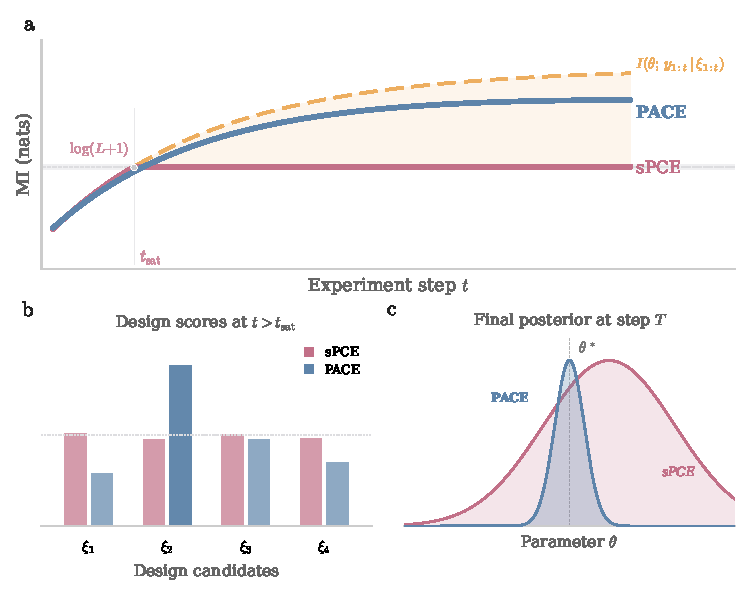
\includegraphics[width=\linewidth]{figures/fig_a1_hero.pdf}
  \caption[The saturation obstacle and the PACE response]{The problem and the response.
  \textbf{(a)} As experiments accumulate, the true information gain keeps rising, but the
  sPCE bound flattens at its $\log(L+1)$ ceiling after a saturation step
  $t_{\mathrm{sat}}$, while PACE continues to track the truth. \textbf{(b)} After
  saturation, sPCE assigns nearly the same score to every candidate design and cannot
  rank them, whereas PACE still separates them. \textbf{(c)} The downstream
  consequence: PACE yields a tighter posterior at the true parameter $\theta^\ast$.}
  \label{fig:hero}
\end{figure}

\section{Research questions}
\label{sec:intro-rqs}

The thesis is organised around one main question and four sub-questions that correspond
to the four contributions.

\medskip
\noindent\textit{Main question: Can sequential Bayesian experimental design be made
feasible and effective on stiff, broad-prior dynamical systems where amortized policy
methods fail?}

\begin{itemize}[leftmargin=*,itemsep=0.2em]
  \item \textbf{RQ1.} When and why does the prior-contrastive sPCE objective, the
  training signal shared by amortized policy methods, fail, and can the failure be
  quantified before any policy is trained?
  \item \textbf{RQ2.} Can a one-time simulation-based posterior estimator supply
  contrastives that escape saturation, and what new cost does this introduce?
  \item \textbf{RQ3.} Does design selection remain valid when the importance weights
  collapse to a single particle?
  \item \textbf{RQ4.} Across a broad suite of systems, when does forward-only
  posterior-contrastive design match or beat amortized policies, and what predicts the
  crossover?
\end{itemize}

\section{Thesis outline}
\label{sec:intro-outline}

Chapter~\ref{sec:related_work} positions PACE against the policy-based,
per-trajectory, and simulation-based-inference literature and states the gap it fills.
Chapter~\ref{sec:methodology} develops the method in full: it sets up sequential BED,
derives the trajectory objective that policy methods optimise and the contrastive
estimators used for evaluation, then presents the saturation diagnosis (RQ1), the PACE
estimator and its cost transfer (RQ2), the analysis of design selection under weight
collapse (RQ3), the forward-only optimiser and its gradient variant, and the evaluation
protocol. Chapter~\ref{sec:results} reports the empirical study on twelve systems
(RQ4), including the ablation that separates the estimator from the optimiser and the
diagnostics that justify trusting the method when the effective sample size is small.
Chapter~\ref{sec:discussion} discusses when PACE should be used, its practical cost,
and its limitations, and Chapter~\ref{sec:conclusion} answers each research question.
Full derivations, system specifications, and additional diagnostics are in the
appendix; the main text is self-contained without it.
